\chapter{Nonlinear least squares}
\label{chap:nls}

\section{Introduction and examples}
\label{nls-intro}

Gretl supports nonlinear least squares (NLS) using a variant of
the Levenberg--Marquardt algorithm.  The user must supply a
specification of the regression function; prior to giving this
specification the parameters to be estimated must be ``declared'' and
given initial values.  Optionally, the user may supply analytical
derivatives of the regression function with respect to each of the
parameters.  If derivatives are not given, the user must instead give
a list of the parameters to be estimated (separated by spaces or
commas), preceded by the keyword \cmd{params}.  The tolerance
(criterion for terminating the iterative estimation procedure) can be
adjusted using the \cmd{set} command.

The syntax for specifying the function to be estimated consists of the
name of the dependent variable, followed by an expression to generate
it. This is illustrated in the following two examples, with
accompanying derivatives.

\begin{code}
# Consumption function from Greene
nls C = alpha + beta * Y^gamma
    deriv alpha = 1
    deriv beta = Y^gamma
    deriv gamma = beta * Y^gamma * log(Y)
end nls

# Nonlinear function from Russell Davidson
nls y = alpha + beta * x1 + (1/beta) * x2
    deriv alpha = 1
    deriv beta = x1 - x2/(beta*beta)
end nls --vcv
\end{code}

Note the command words \cmd{nls} (which introduces the regression
function), \cmd{deriv} (which introduces the specification of a
derivative), and \cmd{end nls}, which terminates the specification and
calls for estimation. If the \cmd{--vcv} flag is appended to the last
line the covariance matrix of the parameter estimates is printed.

\section{Initializing the parameters}
\label{nls-param}

The parameters of the regression function must be given initial values
prior to the \cmd{nls} command. (In the GUI program this may be done
via the menu item ``Variable, Define new variable'').

In some cases, where the nonlinear function is a generalization of (or
a restricted form of) a linear model, it may be convenient to run an
\cmd{ols} and initialize the parameters from the OLS coefficient
estimates.  In relation to the first example above, one might do:
%
\begin{code}
ols C 0 Y
alpha = $coeff(0)
beta = $coeff(Y)
gamma = 1
\end{code}

And in relation to the second example one might do:
%
\begin{code}
ols y 0 x1 x2
alpha = $coeff(0)
beta = $coeff(x1)
\end{code}

\section{NLS dialog window}
\label{nls-gui}

It is probably most convenient to compose the commands for NLS
estimation in the form of a gretl script but you can also do so
interactively, by selecting the item ``Nonlinear Least Squares'' under
the ``Model, Nonlinear models'' menu.  This opens a dialog box where
you can type the function specification (possibly prefaced by
statements to set the initial parameter values) and the derivatives,
if available.  An example of this is shown in
Figure~\ref{fig-nls-dialog}.  Note that in this context you do not
have to supply the \cmd{nls} and \cmd{end nls} tags.

\begin{figure}[htbp]
  \begin{center}
    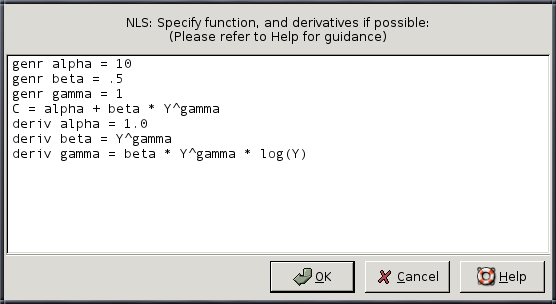
\includegraphics[scale=0.5]{figures/nls_window}
  \end{center}
  \caption{NLS dialog box}
  \label{fig-nls-dialog}
\end{figure}

\section{Analytical and numerical derivatives}
\label{nls-deriv}

If you are able to figure out the derivatives of the regression
function with respect to the parameters, it is advisable to supply
those derivatives as shown in the examples above.  If that is not
possible, gretl will compute approximate numerical derivatives.
However, the properties of the NLS algorithm may not be so good in
this case (see section~\ref{nls-accuracy}).

This is done by using the \cmd{params} statement, which should be
followed by a list of identifiers containing the parameters to be
estimated. In this case, the examples above would read as follows:

\begin{code}
# Greene
nls C = alpha + beta * Y^gamma
    params alpha beta gamma
end nls
\end{code}

\begin{code}
# Davidson
nls y = alpha + beta * x1 + (1/beta) * x2
    params alpha beta
end nls
\end{code}

If analytical derivatives are supplied, they are checked for
consistency with the given nonlinear function.  If the derivatives are
clearly incorrect estimation is aborted with an error message.  If the
derivatives are ``suspicious'' a warning message is issued but
estimation proceeds.  This warning may sometimes be triggered by
incorrect derivatives, but it may also be triggered by a high degree
of collinearity among the derivatives.

Note that you cannot mix analytical and numerical derivatives: you
should supply expressions for all of the derivatives or none.

\section{Advanced use}
\label{sec:nls-generalize}

The \cmd{nls} block can also contain more sophisticated constructs.
First, it can handle intermediate expressions; this makes it possible
to construct the conditional mean expression as a multi-step job, thus
enhancing modularity and readability of the code. Second, more complex
objects, such as lists and matrices, can be used for this purpose.

For example, suppose that we want to estimate a Probit Binary Response
model via NLS. The specification is
\begin{equation}
\label{eq:probit-nls}
y_i = \Phi\left[g(\bm{x}_i)\right] + u_i, \qquad g(\bm{x}_i) = b_0 +
b_1 x_{1,i} + b_2 x_{2,i} = \bm{b}'\bm{x}_i
\end{equation}
Note: this is not the recommended way to estimate a probit model: the
$u_i$ term is heteroskedastic by construction and ML estimation is
much preferable here. Still, NLS is a consistent estimator of the
parameter vector $\bm{b}$, although its covariance matrix will have to
be adjusted to compensate for heteroskedasticity: this is accomplished
via the \option{robust} switch.

\begin{script}[htbp]
  \scriptcaption{NLS estimation of a Probit model}
  \label{script:nls-probit-numder}
  \begin{scode}
    open greene25_1.gdt
    list X = const age income ownrent selfempl

    # initalisation
    ols cardhldr X --quiet
    matrix b = $coeff / $sigma

    # proceed with NLS estimation
    nls cardhldr = cnorm(ndx)
        series ndx = lincomb(X, b)
        params b
    end nls --robust

    # compare with ML probit 
    probit cardhldr X --p-values
  \end{scode}
\end{script}

The example in script \ref{script:nls-probit-numder} can be enhanced by
using analytical derivatives: since
\[
\frac{\partial g(\bm{x}_i)}{\partial b_j} = \varphi(\bm{b}'\bm{x}_i) \cdot x_{ij}
\]
one could substitute the \cmd{params} line in the script with the two-liner
\begin{code}
  series f = dnorm(ndx)
  deriv b = {f} .* {X}
\end{code}
and have \cmd{nls} use analytically-computed derivatives, which are
quicker and usually more reliable.

\section{Controlling termination}
\label{nls-toler}

The NLS estimation procedure is an iterative process.  Iteration is
terminated when the criterion for convergence is met or when the
maximum number of iterations is reached, whichever comes first.

Let $k$ denote the number of parameters being estimated.  The maximum
number of iterations is $100 \times (k+1)$ when analytical derivatives
are given, and $200 \times (k+1)$ when numerical derivatives are used.

Let $\epsilon$ denote a small number.  The iteration is deemed to have
converged if at least one of the following conditions is satisfied:

\begin{itemize}
\item Both the actual and predicted relative reductions in the error
  sum of squares are at most $\epsilon$.
\item The relative error between two consecutive iterates is at most
  $\epsilon$.
\end{itemize}

This default value of $\epsilon$ is the machine precision to the power
3/4,\footnote{On a 32-bit Intel Pentium machine a likely value for
  this parameter is $1.82\times 10^{-12}$.} but it can be adjusted
using the \cmd{set} command with the parameter \verb+nls_toler+.  For
example
%
\begin{code}
set nls_toler .0001
\end{code}
% 
will relax the value of $\epsilon$ to 0.0001.

\section{Details on the code}
\label{nls-code}

The underlying engine for NLS estimation is based on the \app{minpack}
suite of functions, available from
\href{http://www.netlib.org/minpack/}{netlib.org}.  Specifically, the
following \app{minpack} functions are called:

\begin{center}
  \begin{tabular}{ll}
    \verb+lmder+ & Levenberg--Marquardt algorithm with analytical
    derivatives
    \\
    \verb+chkder+ & Check the supplied analytical derivatives
    \\
    \verb+lmdif+ & Levenberg--Marquardt algorithm with numerical
    derivatives
    \\
    \verb+fdjac2+ & Compute final approximate Jacobian when using
    numerical derivatives
    \\
    \verb+dpmpar+ & Determine the machine precision
    \\
  \end{tabular}
\end{center}

On successful completion of the Levenberg--Marquardt iteration, a
Gauss--Newton regression is used to calculate the covariance matrix
for the parameter estimates.  If the \option{robust} flag is given a
robust variant is computed.  The documentation for the \cmd{set}
command explains the specific options available in this regard.

Since NLS results are asymptotic, there is room for debate over
whether or not a correction for degrees of freedom should be applied
when calculating the standard error of the regression (and the
standard errors of the parameter estimates).  For comparability with
OLS, and in light of the reasoning given in
\cite{davidson-mackinnon93}, the estimates shown in gretl
\emph{do} use a degrees of freedom correction.

\section{Numerical accuracy}
\label{nls-accuracy}

Table \ref{tab-nls} shows the results of running the gretl NLS
procedure on the 27 Statistical Reference Datasets made available by
the U.S.  National Institute of Standards and Technology (NIST) for
testing nonlinear regression software.\footnote{For a discussion of
  gretl's accuracy in the estimation of linear models, see
  Appendix~\ref{app-accuracy}.}  For each dataset, two sets of
starting values for the parameters are given in the test files, so the
full test comprises 54 runs.  Two full tests were performed, one using
all analytical derivatives and one using all numerical approximations.
In each case the default tolerance was used.\footnote{The data shown
  in the table were gathered from a pre-release build of gretl
  version 1.0.9, compiled with \app{gcc} 3.3, linked against
  \app{glibc} 2.3.2, and run under Linux on an i686 PC (IBM ThinkPad
  A21m).}

Out of the 54 runs, gretl failed to produce a solution
in 4 cases when using analytical derivatives, and in 5 cases when
using numeric approximation. Of the four failures in analytical
derivatives mode, two were due to non-convergence of the
Levenberg--Marquardt algorithm after the maximum number of iterations
(on \verb+MGH09+ and \verb+Bennett5+, both described by NIST as of
``Higher difficulty'') and two were due to generation of range errors
(out-of-bounds floating point values) when computing the Jacobian (on
\verb+BoxBOD+ and \verb+MGH17+, described as of ``Higher difficulty''
and ``Average difficulty'' respectively).  The additional failure in
numerical approximation mode was on \verb+MGH10+ (``Higher
difficulty'', maximum number of iterations reached).

The table gives information on several aspects of the tests: the
number of outright failures, the average number of iterations taken to
produce a solution and two sorts of measure of the accuracy of the
estimates for both the parameters and the standard errors of the
parameters.

For each of the 54 runs in each mode, if the run produced a solution
the parameter estimates obtained by gretl were compared with the
NIST certified values.  We define the ``minimum correct figures'' for
a given run as the number of significant figures to which the
\emph{least accurate} gretl estimate agreed with the certified
value, for that run. The table shows both the average and the worst
case value of this variable across all the runs that produced a
solution.  The same information is shown for the estimated standard
errors.\footnote{For the standard errors, I excluded one outlier from
  the statistics shown in the table, namely \verb+Lanczos1+.  This is
  an odd case, using generated data with an almost-exact fit: the
  standard errors are 9 or 10 orders of magnitude smaller than the
  coefficients.  In this instance gretl could reproduce the
  certified standard errors to only 3 figures (analytical derivatives)
  and 2 figures (numerical derivatives).}  

The second measure of accuracy shown is the percentage of cases,
taking into account all parameters from all successful runs, in which
the gretl estimate agreed with the certified value to at least
the 6 significant figures which are printed by default in the
gretl regression output.

\begin{table}[htbp]
 \caption{Nonlinear regression: the NIST tests}
 \label{tab-nls}
  \begin{center}
    \begin{tabular}{lcc}
      & \textit{Analytical derivatives} & 
      \textit{Numerical derivatives} \\ [4pt]
        Failures in 54 tests & 4 & 5\\
        Average iterations & 32 & 127\\
        Mean of min. correct figures, & 8.120 & 6.980\\
        parameters \\
        Worst of min. correct figures, & 4 & 3\\
        parameters \\
        Mean of min. correct figures, & 8.000 & 5.673\\
        standard errors \\
        Worst of min. correct figures, & 5 & 2\\
        standard errors \\
        Percent correct to at least 6 figures, & 96.5 & 91.9\\
        parameters \\
        Percent correct to at least 6 figures, & 97.7 & 77.3\\
        standard errors \\
      \end{tabular}
    \end{center}
  \end{table}

  Using analytical derivatives, the worst case values for both
  parameters and standard errors were improved to 6 correct figures on
  the test machine when the tolerance was tightened to 1.0e$-$14.
  Using numerical derivatives, the same tightening of the tolerance
  raised the worst values to 5 correct figures for the parameters and
  3 figures for standard errors, at a cost of one additional failure
  of convergence.

  Note the overall superiority of analytical derivatives: on average
  solutions to the test problems were obtained with substantially
  fewer iterations and the results were more accurate (most notably
  for the estimated standard errors).  Note also that the six-digit
  results printed by gretl are not 100 percent reliable for
  difficult nonlinear problems (in particular when using numerical
  derivatives).  Having registered this caveat, the percentage of
  cases where the results were good to six digits or better seems high
  enough to justify their printing in this form.

%%% Local Variables: 
%%% mode: latex
%%% TeX-master: "gretl-guide"
%%% End: 
